\chapter{}\label{sec:appendix_mydata}

\begin{figure}[h]
  \begin{subfigure}[b]{0.42\textwidth}
    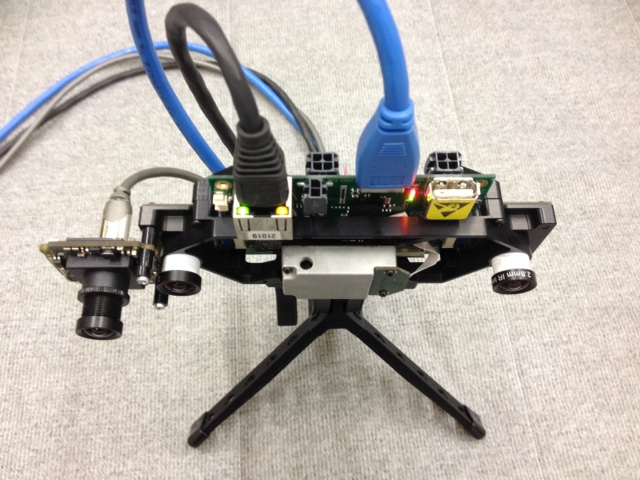
\includegraphics[width=\textwidth]{images/vi_bluefox.JPG}
    \caption{}
  \end{subfigure}
  \hfill
  \begin{subfigure}[b]{0.42\textwidth}
    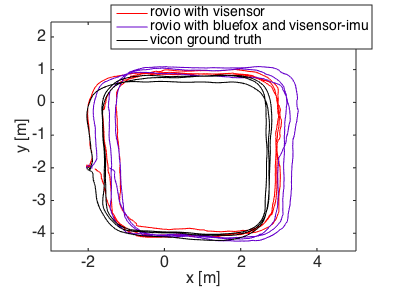
\includegraphics[width=\textwidth]{images/slow_2D.png}
    \caption{}
  \end{subfigure}
  \hfill
  \begin{subfigure}[b]{0.42\textwidth}
    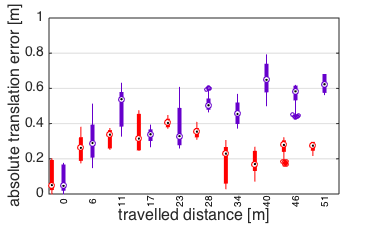
\includegraphics[width=\textwidth]{images/slow/slow_ate.png}
    \caption{}
  \end{subfigure}
  \begin{subfigure}[b]{0.42\textwidth}
    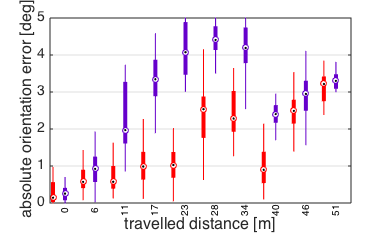
\includegraphics[width=\textwidth]{images/slow/slow_aoe.png}
    \caption{}
  \end{subfigure}
  \hfill
  \begin{subfigure}[b]{0.42\textwidth}
    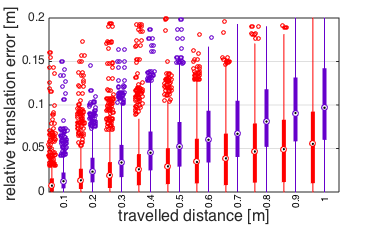
\includegraphics[width=\textwidth]{images/slow/slow_rte.png}
    \caption{}
  \end{subfigure}
  \hfill
  \begin{subfigure}[b]{0.42\textwidth}
    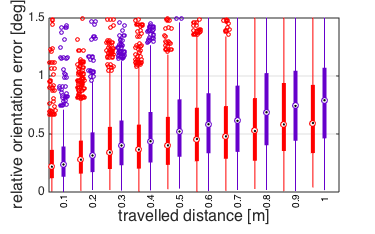
\includegraphics[width=\textwidth]{images/slow/slow_roe.png}
    \caption{}
  \end{subfigure}
   \caption{ROVIO results on the slow dataset with dynamics of $1.5\frac{m}{s}$ and $1\frac{rad}{s}$. ROVIO's tracking performance on the VI-sensor data (hardware-wise time synchronized) is better than on the data of the bluefox camera and the VI-sensor-IMU (hardware-wise non time synchronized). ROVIO is principally able to track for both the time synchronized and the non time synchronized data.}
   \label{pics:appendix_slow}
\end{figure}

\begin{figure}[h]
  \begin{subfigure}[b]{0.42\textwidth}
    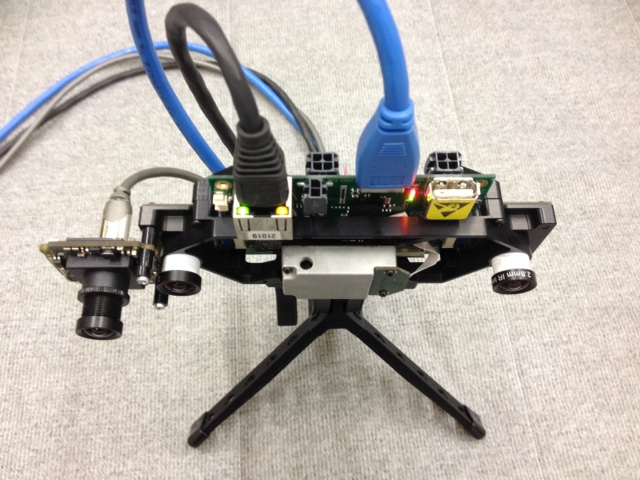
\includegraphics[width=\textwidth]{images/vi_bluefox.JPG}
    \caption{}
  \end{subfigure}
  \hfill
  \begin{subfigure}[b]{0.42\textwidth}
    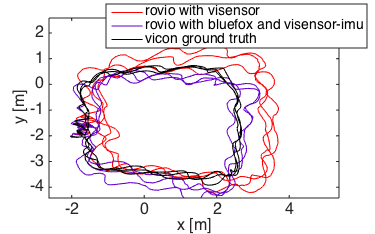
\includegraphics[width=\textwidth]{images/fast_fixed_2D.png}
    \caption{}
  \end{subfigure}
  \hfill
  \begin{subfigure}[b]{0.42\textwidth}
    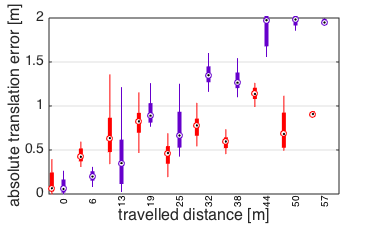
\includegraphics[width=\textwidth]{images/fast_fixed/fast_fixed_ate.png}
    \caption{}
  \end{subfigure}
  \begin{subfigure}[b]{0.42\textwidth}
    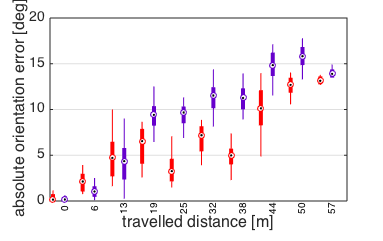
\includegraphics[width=\textwidth]{images/fast_fixed/fast_fixed_aoe.png}
    \caption{}
  \end{subfigure}
  \hfill
  \begin{subfigure}[b]{0.42\textwidth}
    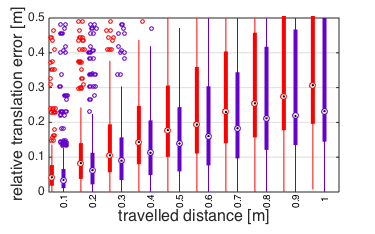
\includegraphics[width=\textwidth]{images/fast_fixed/fast_fixed_rte.png}
    \caption{}
  \end{subfigure}
  \hfill
  \begin{subfigure}[b]{0.42\textwidth}
    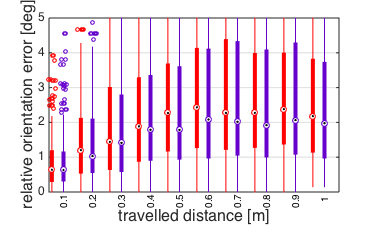
\includegraphics[width=\textwidth]{images/fast_fixed/fast_fixed_roe.png}
    \caption{}
  \end{subfigure}
   \caption{ROVIO results on the fast dataset with dynamics of $2.5\frac{m}{s}$ and $5\frac{rad}{s}$ and fixed extrinsics between camera and IMU. As demonstrated in section \ref{sec:timesync} ROVIO is diverging on this dataset when the extrinsics between camera and IMU are estimated online. By fixing the extrinsics on the hardware-wise non time synchronized setup ROVIO is not diverging anymore. The global tracking performance is still worse than the one of ROVIO running on the VI-sensor data, the local tracking performance is even slightly better than the one of ROVIO running on the VI-sensor data. This dataset is lying at the dynamic limits of ROVIO and the local accuracy on both the time synchronized and non time synchronized data is low.}
   \label{pics:appendix_fast}
\end{figure}